\lab{K-Means Clustering}{K-Means Clustering}
\objective{Understand the basics of \emph{k-means} clustering, and apply to the problem of clustering earthquake epicenters.}

\subsection*{Clustering}
In Lab \ref{lab:pca}, we analyzed the iris dataset using PCA; we have reproduced the first two principal components of the iris data in Figure \ref{fig:iris_data}. 
Upon inspection of the first two principal components, a human can easily see that there are two very distinct groups of irises. 
Can we create an algorithm to identify these groups without human supervision? 
This task is called \emph{clustering}, an instance of \emph{unsupervised learning}.

\begin{figure}
\centering
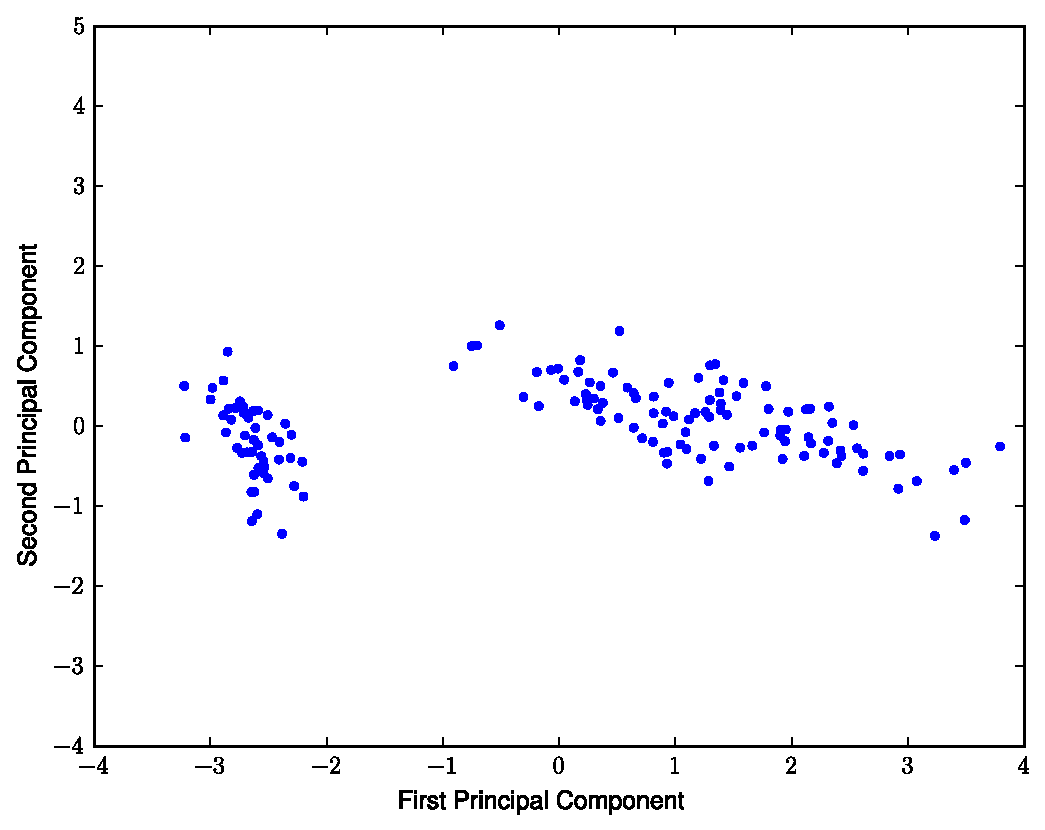
\includegraphics[width=\textwidth]{iris_pca.pdf}
\caption{The first two principal components of the iris dataset.}
\label{fig:iris_data}
\end{figure}

The objective of clustering is to find a partition of the data such that points in the same subset will be ``close'' according to some metric. 
The metric used will likely depend on the data, but some obvious choices include Euclidean distance and angular distance. 
Throughout this lab we will use the metric $d(x,y) = \|x-y\|_2$, the Euclidean distance between $x$ and $y$.

More formally, suppose we have a collection of $\mathbb{R}^K$-valued observations $X = \{x_1,x_2,\ldots,x_n\}$. 
Let $N \in \mathbb{N}$ and let $\mathcal{S}$ be the set of all $N$-partitions of $X$, where an $N$-partition is a partition with exactly $N$ nonempty elements.
We can represent a typical partition in $\mathcal{S}$ as $S = \{S_1,S_2,\ldots,S_N\}$, where
\[
X = \bigcup_{i=1}^N S_i
\] 
and
\[
|S_i| > 0, \qquad i=1,2,\ldots,N.
\]
We seek the $N$-partition $S^*$ that minimizes the within-cluster sum of squares, i.e.
\[
S^* = \underset{S\in\mathcal{S}}{\arg\min} \sum_{i=1}^N\sum_{x_j\in S_i}\|x_j-\mu_i\|_2^2,
\]
where $\mu_i$ is the mean of the elements in $S_i$, i.e.
\[
\mu_i = \frac{1}{|S_i|}\sum_{x_j\in S_i}x_j.
\]

\subsection*{The \emph{K-Means} Method}
Finding the global minimizing partition $S^*$ is generally intractable since the set of partitions can be very large indeed, 
but the \emph{k-means} algorithm is a heuristic approach that can often provide good results.


We begin by specifying an initial cluster mean $\mu_i^{(1)}$ for each $i = 1, \cdots, N$ (this can be done by random initialization, or according to some heuristic).
For each iteration, we adopt the following procedure. 
Given a current set of cluster means $\mu^{(t)}$, we find a partition $S^{(t)}$ of the observations such that
\begin{equation*}
S_{i}^{(t)} = \{x_j \; : \; \|x_j - \mu_{i}^{(t)}\|_2^2 \leq \|x_j - \mu_{l}^{(t)}\|_2^2,\,\,\,  l = 1, \cdots, N\}.
\end{equation*}
We then update our cluster means by computing for each $i = 1, \cdots, N$.
We continue to iterate in this manner until the partition ceases to change. 



Examine Figure \ref{fig:iris_clusterings}, which shows two different clusterings of the iris data produced by the \emph{k-means} algorithm.
Note that the quality of the clustering can depend heavily on the initial cluster means.
We can use the within-cluster sum of squares as a measure of the quality of a clustering (a lower sum of squares is better).
Where possible, it is advisable to run the clustering algorithm several times, each with a different initialization of the means,
and keep the best clustering. 
Note also that it is possible to have very slow convergence.
Thus, when implementing the algorithm, it is a good idea to terminate after some specified maximum number of iterations.

\begin{figure}[h]
	\centering
	\begin{tabular}{cc}
	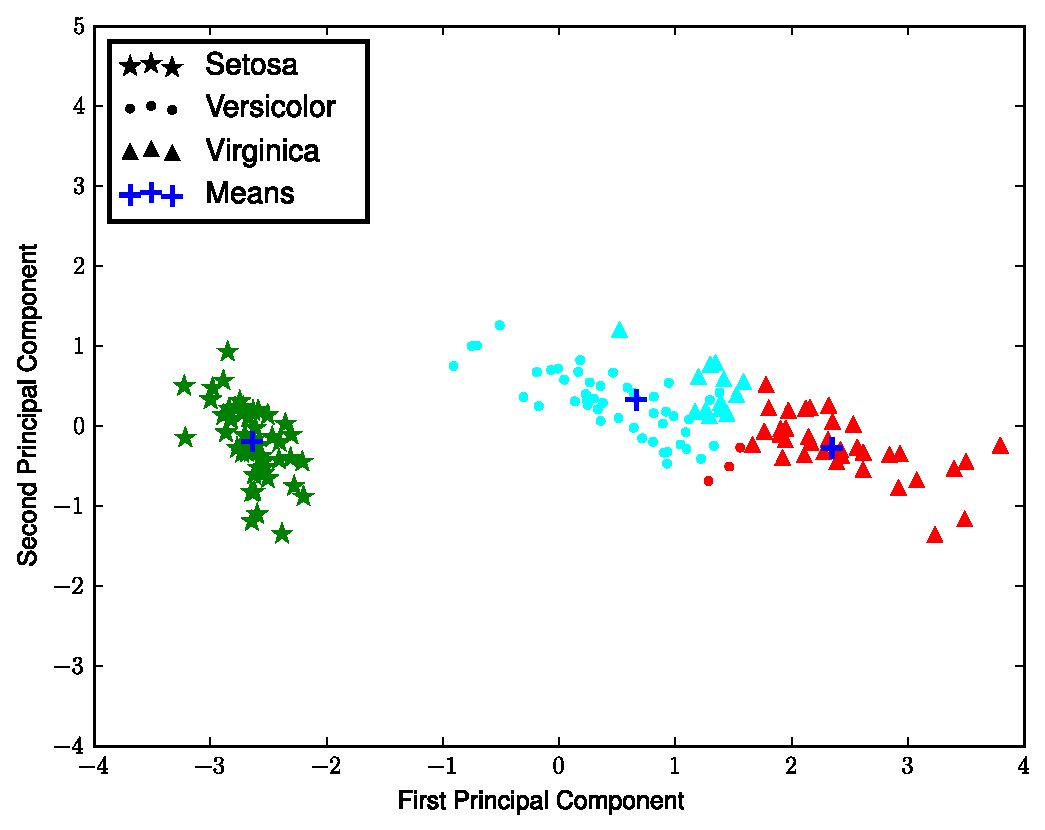
\includegraphics[width=.49\textwidth]{iris_means_1.pdf} &
	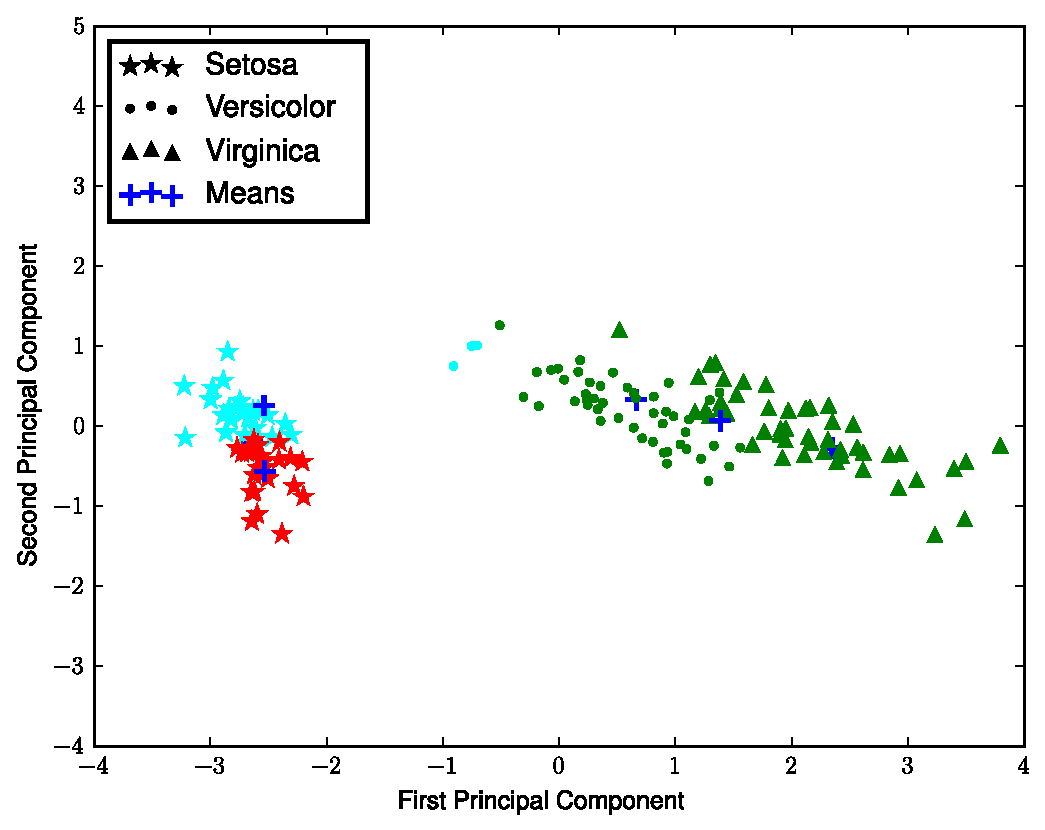
\includegraphics[width=.49\textwidth]{iris_means_2.pdf} 
	\end{tabular}
	\caption{Two different K-Means clusterings for the iris dataset. 
            Notice that the clustering on the left predicts the flower species to a high degree of accuracy,
            while the clustering on the right is less effective.}
    \label{fig:iris_clusterings}
\end{figure}

\begin{problem}
Implement the \emph{k-means} algorithm using the following function declaration.

\begin{lstlisting}
def kmeans(data,n_clusters,init='random',max_iter=300):
    """
    Cluster a dataset using the k-means algorithm.
    
    Parameters
    ----------
    data : ndarray of shape (n,k)
        Each row is an observation.
    n_clusters : int
        The number of clusters.
    init : string or ndarray of shape (n_clusters,k)
        If init is the string 'random', then randomly initialize the cluster means.
        Else, the initial cluster means are given by the rows of init.
    max_iter : int
        The maximum allowable number of iterations.
        
    Returns
    -------
    means : ndarray of shape (n_cluster,k)
        The final cluster means, given as the rows.
    labels : ndarray of shape (n,)
        The i-th entry is an integer in [0,n_clusters-1] indicating 
        which cluster the i-th row of data belongs to relative to 
        the rows of means.
    measure : float
        The within-cluster sum of squares quality measure.
    """
    pass
\end{lstlisting} 

Test your function on the first two principal components of the iris dataset. 
Run it 10 times, using a different random initialization of the means each time.
Retain the clustering with the smallest within-cluster sum of squares.
Your clustering should be similar to the first clustering in Figure \ref{fig:iris_clusterings}.
\end{problem}

\subsection*{Detecting Active Earthquake Regions}

Suppose we are interested in learning about which regions are prone to experience frequent earthquake activity. We could make a map of all earthquakes over a given period of time and examine it ourselves, but we recognize this as an unsupervised learning problem and are eager to apply our new k-means clustering tool.

We have 6 .txt files, each containing a months worth of earthquake data throughout the world, from January 2010 through June 2010. These files contain a lot of information which we aren't interested in at the time; all we would like to extract from them is the location of each earthquake, which appears in characters $21$ through $33$ of each line. Characters $21$ through $26$ contain the latitude of each epicenter, character $26$ denoting North or South, and characters $27$ through $33$ contain the longitude of each epicenter, character $33$ denoting East or West. We need to divide each value by $1,000$ to represent these as degrees and decimals.

We might think that we can regard any epicenter as a point in $\mathbb{R}^{2}$ with coordinates being their latitude and longitude. This, however, would be incorrect, because the earth is not flat. We must recognize that latitude and longitude are best viewed as a variation of spherical coordinates in $\mathbb{R}^{3}$, and we should interpret them as such. Each point in $\mathbf{R}^{3}$ can be represented in Euclidean coordinates as a triple $(x,y,z)$, or in spherical coordinates as a triple $(r,\theta,\phi)$, where $r$ is the distance from the origin, $\theta$ is the angle made with the $z$-axis, and $\phi$ is the angle made by the projection onto the $x-y$ plane and the $x$-axis. Because we are considering a sphere (the earth), we can assume its radius is $1$, and ignore it throughout.

\begin{problem}
Write a function which accepts a file name of earthquake data and extracts the latitude and longitude of each earthquake epicenter. Transform these coordinates into spherical coordinates. To do this, we have to recognize that in spherical coordinates, the polar angle is measured from the north pole, not from the equator, being a transformation of the latitudes. See the figures below. The longitudes should not require a transformation. Write another function that does this for all files in the directory containing the earthquake data and returns all epicenters in spherical coordinates, with $r = 1$.
\end{problem}

\begin{figure}[h]
\centering
	\begin{tabular}{cc}
		\includegraphics[width=.49\textwidth]{latlong.png}
		\includegraphics[width=.49\textwidth]{spherical.png}
	\end{tabular}
	\caption{Longitude and Latitude vs. Spherical Coordinates}
\end{figure}

Recall the transformations from spherical coordinates to Euclidean coordinates, and vice-versa:
\begin{align*}
r & = \sqrt{x^{2} + y^{2} + z^{2}} & x & = r \sin \theta \cos \phi \\
\theta & = \arccos \frac{z}{r} & y & = r \sin \theta \sin \phi \\
\phi & = \arctan \frac{y}{x} & z & = r \cos \theta
\end{align*}

\begin{problem}
Write three functions, one that transforms data from spherical coordinates to Euclidean coordinates, another that reverses this transformation, and a third which transforms data from spherical coordinates to latitude and longitude.
\end{problem}

\begin{problem}
Load all of the earthquake epicenters data and transform them into Euclidean coordinates in $\mathbb{R}^{3}$. Cluster the earthquakes into $15$ clusters, being sure to normalize your centroids at each step (thus keeping the earthquakes on the surface of the earth).
\end{problem}

\begin{problem}
Transform your epicenters data and your final centroids into latitude and longitude pairs and plot each cluster with a different color, as well as each centroid with a ``+'' symbol as before. You should be able to recognize geographical features (North America, the Asian Pacific coast, etc.), and see different regions of earthquake activity as in Figure \ref{fig:earthquakeclusters}.
\end{problem}

\begin{figure}
	\centering
	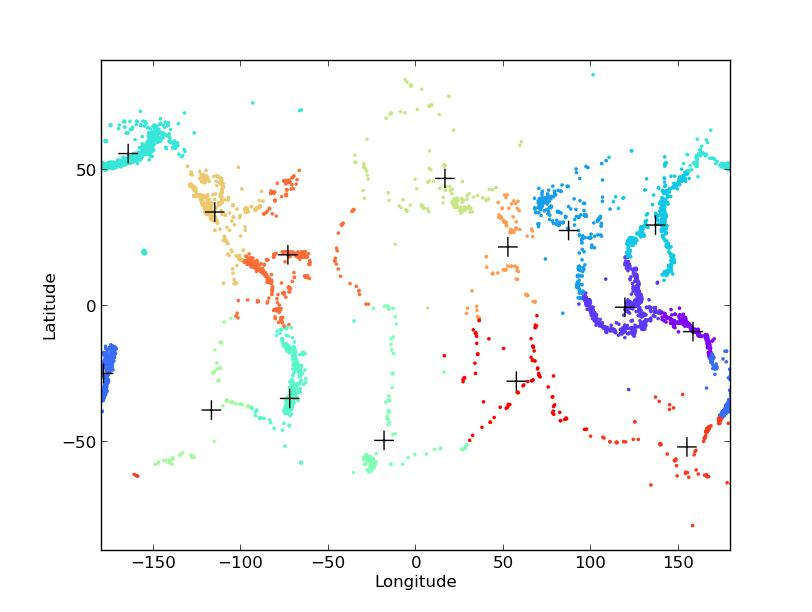
\includegraphics[width=\textwidth]{clusters.jpg}
	\caption{Earthquake epicenter clusters with $N = 15$}
	\label{fig:earthquakeclusters}
\end{figure}
